\chapter{HASIL DAN PEMBAHASAN}
\label{chap:hasilpembahasan}
\setlength{\belowcaptionskip}{-5pt}
% Ubah bagian-bagian berikut dengan isi dari hasil dan pembahasan
Pada penelitian ini, dipaparkan hasil pengujian serta analisis dari desain sistem dan implementasi. Data yang digunakan dalam pengujian diambil dari kamera handphone. Pengambilan data yang digunakan adalah gambar tulisan tangan sendiri dan tulisan orang lain. Dipaparkan skenario pengujian hasil training, pada tahapan skenario pengujian terdapat 4 jenis pengujian yaitu:

\begin{enumerate}[nolistsep, topsep=0pt]
	\item Pengujian menggunakan tulisan orang lain.
	\item Pengujian menggunakan jarak pengambilan gambar, yaitu:
	\begin{itemize}
		\item Jarak pengambilan gambar 40cm
		\item Jarak pengambilan gambar 60cm
		\item Jarak pengambilan gambar 80cm
	\end{itemize}
	\item Pengujian menggunakan warna spidol berbeda, yaitu:
	\begin{itemize}
		\item Warna spidol biru
		\item Warna spidol merah
		\item Warna spidol hijau
	\end{itemize}
	\item Pengujian menggunakan gambar bangun datar yang diarsir.
\end{enumerate}

\section{Pengujian Menggunakan Tulisan Orang Lain}
Pada tahap pengujian ini, data yang digunakan adalah gambar bangun datar beserta parameternya dari tulisan tangan orang lain. Setelah itu dilakukan deteksi objek bangun datar beserta parameternya, dilanjutkan dengan perhitungan luas. Pengujian ini bermaksud untuk melihat seberapa berhasilnya bila model yang sudah di training pada tahap \ref{subsec: Training} di uji coba menggunakan tulisan tangan orang lain. berikut pada gambar \ref{fig:segitigaoranglain} sampai \ref{fig:trapesiumoranglain} adalah hasilnya.
\begin{center}
	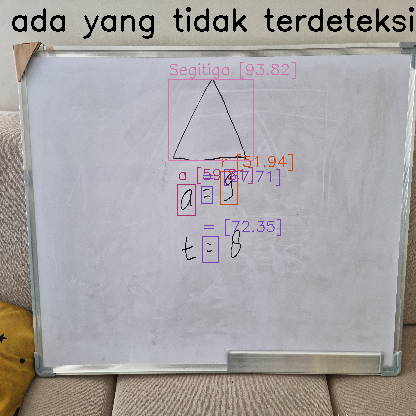
\includegraphics[width=0.55\textwidth]{gambar/segitiga orang.png}
	\captionof{figure}{Deteksi Segitiga Menggunakan Tulisan Orang Lain}
	\label{fig:segitigaoranglain}
\end{center}
Pada Gambar \ref{fig:segitigaoranglain} didapatkan tidak sepenuhnya berhasil deteksi daripada gambar bangun datar segitiga beserta parameter huruf dan angka, yang mengakibatkan tidak berhasilnya perhitungan luas yang mana hasil dari gagalnya perhitungan luas diletakkan pada pojok kiri atas \textit{window} gambar dengan penjelasan "ada yang tidak terdeteksi".

\begin{center}
	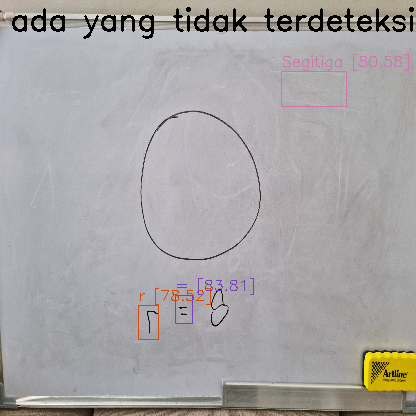
\includegraphics[width=0.55\textwidth]{gambar/lingkaran orang.png}
	\captionof{figure}{Deteksi Lingkaran Menggunakan Tulisan Orang Lain}
	\label{fig:lingkaranoranglain}
\end{center}
Pada Gambar \ref{fig:lingkaranoranglain} didapatkan tidak sepenuhnya berhasil deteksi daripada gambar bangun datar lingkaran beserta parameter huruf dan angka, yang mengakibatkan tidak berhasilnya perhitungan luas yang mana hasil dari gagalnya perhitungan luas diletakkan pada pojok kiri atas \textit{window} gambar dengan penjelasan "ada yang tidak terdeteksi".

\begin{center}
	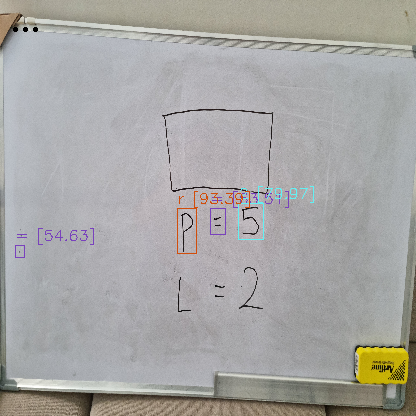
\includegraphics[width=0.55\textwidth]{gambar/persegipanjang orang.png}
	\captionof{figure}{Deteksi Persegi Panjang Menggunakan Tulisan Orang Lain}
	\label{fig:persegipanjangoranglain}
\end{center}
Pada Gambar \ref{fig:persegipanjangoranglain} didapatkan tidak sepenuhnya berhasil deteksi daripada gambar bangun datar persegi panjang beserta parameter huruf dan angka, yang mengakibatkan tidak berhasilnya perhitungan luas yang mana hasil dari gagalnya perhitungan luas diletakkan pada pojok kiri atas \textit{window} gambar dengan penjelasan "...".

\begin{center}
	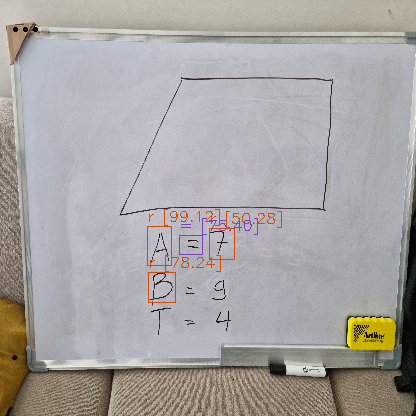
\includegraphics[width=0.55\textwidth]{gambar/trapesium orang.png}
	\captionof{figure}{Deteksi Trapesium Menggunakan Tulisan Orang Lain}
	\label{fig:trapesiumoranglain}
\end{center}
Pada Gambar \ref{fig:trapesiumoranglain} didapatkan tidak sepenuhnya berhasil deteksi daripada gambar bangun datar trapesium beserta parameter huruf dan angka, yang mengakibatkan tidak berhasilnya perhitungan luas yang mana hasil dari gagalnya perhitungan luas diletakkan pada pojok kiri atas \textit{window} gambar dengan penjelasan "...".

\section{Pengujian menggunakan jarak pengambilan gambar yang berbeda}
\label{sec:Hasil Metodologi}
Pada pengujian menggunakan ukuran tulisan yang berbeda dilakukan pengujian menggunakan tulisan tangan si peneliti dengan jarak pengambilan gambar yang berbeda, setelah itu dilakukan deteksi objek bangun datar beserta parameternya, dilanjutkan dengan perhitungan luas. Pengujian ini bermaksud untuk melihat seberapa berhasilnya bila model yang sudah di training pada tahap \ref{subsec: Training} di uji coba menggunakan ukuran tulisan atau jarak pengambilan gambar yang berbeda. Jarak yang digunakan dalam pengujian ini adalah:
\begin{itemize}
	\item Jarak pengambilan gambar 40cm.
	\item Jarak pengambilan gambar 60cm.
	\item Jarak pengambilan gambar 80cm.
\end{itemize}

\subsection{Jarak Pengambilan Gambar 40cm}
\begin{center}
	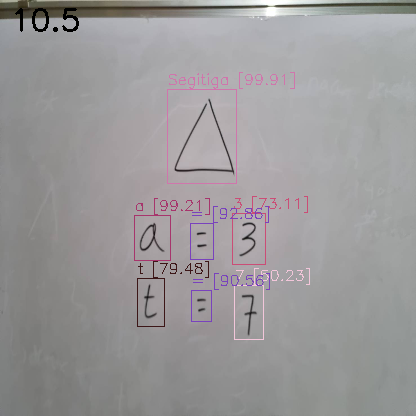
\includegraphics[width=0.55\textwidth]{gambar/segitiga2.png}
	\captionof{figure}{Deteksi Segitiga dan Hasilnya Pada Pengambilan Gambar 40cm}
	\label{fig:segitigatest2}
\end{center}
Pada Gambar \ref{fig:segitigatest2} didapatkan berhasilnya deteksi daripada gambar bangun datar segitiga beserta parameter huruf dan angka, yang mengakibatkan berhasilnya perhitungan luas yang mana hasil dari perhitungan luas diletakkan pada pojok kiri atas \textit{window} gambar.

\begin{center}
	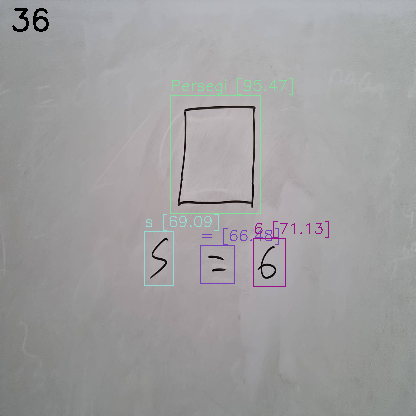
\includegraphics[width=0.55\textwidth]{gambar/persegi2.png}
	\captionof{figure}{Deteksi Persegi dan Hasilnya Pada Pengambilan Gambar 40cm}
	\label{fig:persegitest2}
\end{center}
Pada Gambar \ref{fig:persegitest2} didapatkan berhasilnya deteksi daripada gambar bangun datar persegi beserta parameter huruf dan angka, yang mengakibatkan berhasilnya perhitungan luas yang mana hasil dari perhitungan luas diletakkan pada pojok kiri atas \textit{window} gambar.

\begin{center}
	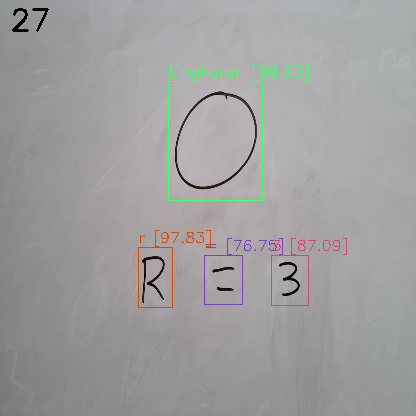
\includegraphics[width=0.55\textwidth]{gambar/lingkaran2.png}
	\captionof{figure}{Deteksi Lingkaran dan Hasilnya Pada Pengambilan Gambar 40cm}
	\label{fig:lingkarantest2}
\end{center}
Pada Gambar \ref{fig:lingkarantest2} didapatkan berhasilnya deteksi daripada gambar bangun datar lingkaran beserta parameter huruf dan angka, yang mengakibatkan berhasilnya perhitungan luas yang mana hasil dari perhitungan luas diletakkan pada pojok kiri atas \textit{window} gambar.

\begin{center}
	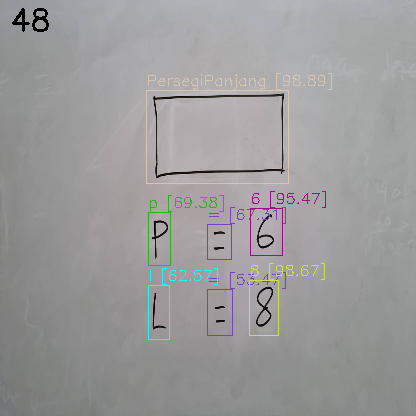
\includegraphics[width=0.55\textwidth]{gambar/persegi panjang2.png}
	\captionof{figure}{Deteksi Persegi Panjang dan Hasilnya Pada Pengambilan Gambar 40cm}
	\label{fig:persegipanjangtest2}
\end{center}
Pada Gambar \ref{fig:persegipanjangtest2} didapatkan berhasilnya deteksi daripada gambar bangun datar persegi panjang beserta parameter huruf dan angka, yang mengakibatkan berhasilnya perhitungan luas yang mana hasil dari perhitungan luas diletakkan pada pojok kiri atas \textit{window} gambar.

\begin{center}
	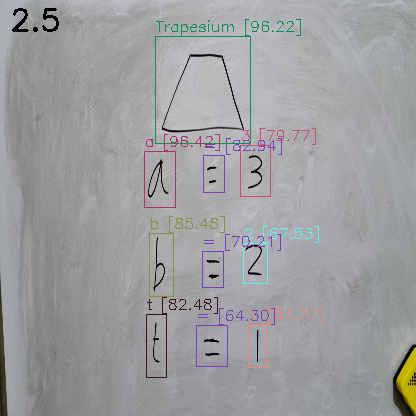
\includegraphics[width=0.55\textwidth]{gambar/trapesium2.png}
	\captionof{figure}{Deteksi Trapesium dan Hasilnya Pada Pengambilan Gambar 40cm}
	\label{fig:trapesiumtest2}
\end{center}
Pada Gambar \ref{fig:trapesiumtest2} didapatkan berhasilnya deteksi daripada gambar bangun datar trapesium beserta parameter huruf dan angka, yang mengakibatkan berhasilnya perhitungan luas yang mana hasil dari perhitungan luas diletakkan pada pojok kiri atas \textit{window} gambar.

\subsection{Jarak Pengambilan Gambar 60cm}
\begin{center}
	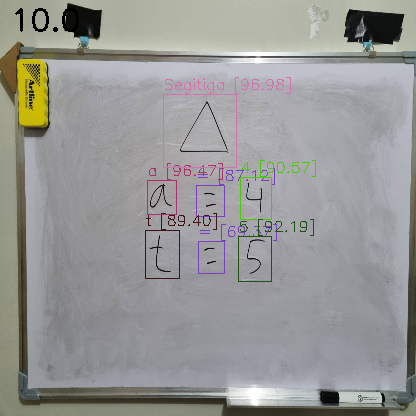
\includegraphics[width=0.55\textwidth]{gambar/seg60hasil.png}
	\captionof{figure}{Deteksi Segitiga dan Hasilnya Pada Pengambilan Gambar 60cm}
	\label{fig:segitigatest60}
\end{center}
Pada Gambar \ref{fig:segitigatest60} didapatkan berhasilnya deteksi daripada gambar bangun datar segitiga beserta parameter huruf dan angka, yang mengakibatkan berhasilnya perhitungan luas yang mana hasil dari perhitungan luas diletakkan pada pojok kiri atas \textit{window} gambar.

\begin{center}
	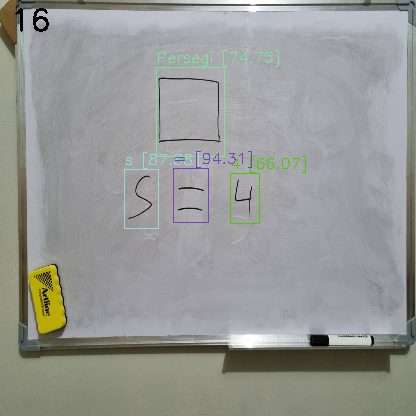
\includegraphics[width=0.55\textwidth]{gambar/pers60hasil.png}
	\captionof{figure}{Deteksi Persegi dan Hasilnya Pada Pengambilan Gambar 60cm}
	\label{fig:persegitest60}
\end{center}
Pada Gambar \ref{fig:persegitest60} didapatkan berhasilnya deteksi daripada gambar bangun datar persegi beserta parameter huruf dan angka, yang mengakibatkan berhasilnya perhitungan luas yang mana hasil dari perhitungan luas diletakkan pada pojok kiri atas \textit{window} gambar.

\begin{center}
	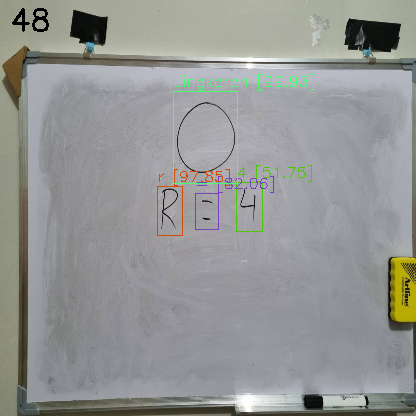
\includegraphics[width=0.55\textwidth]{gambar/ling60hasil.png}
	\captionof{figure}{Deteksi Lingkaran dan Hasilnya Pada Pengambilan Gambar 60cm}
	\label{fig:lingkarantest60}
\end{center}
Pada Gambar \ref{fig:lingkarantest60} didapatkan berhasilnya deteksi daripada gambar bangun datar lingkaran beserta parameter huruf dan angka, yang mengakibatkan berhasilnya perhitungan luas yang mana hasil dari perhitungan luas diletakkan pada pojok kiri atas \textit{window} gambar.

\begin{center}
	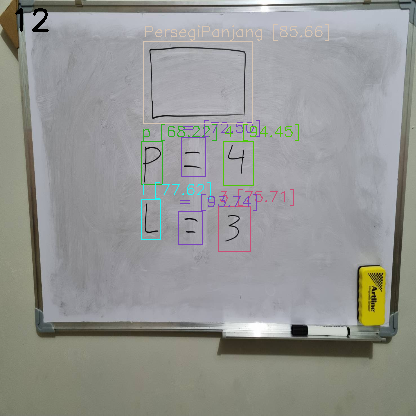
\includegraphics[width=0.55\textwidth]{gambar/pp60hasil.png}
	\captionof{figure}{Deteksi Persegi Panjang dan Hasilnya Pada Pengambilan Gambar 60cm}
	\label{fig:persegipanjangtest60}
\end{center}
Pada Gambar \ref{fig:persegipanjangtest60} didapatkan berhasilnya deteksi daripada gambar bangun datar persegi panjang beserta parameter huruf dan angka, yang mengakibatkan berhasilnya perhitungan luas yang mana hasil dari perhitungan luas diletakkan pada pojok kiri atas \textit{window} gambar.

\begin{center}
	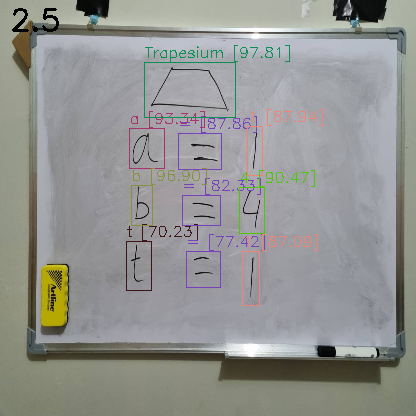
\includegraphics[width=0.55\textwidth]{gambar/trap60hasil.png}
	\captionof{figure}{Deteksi Trapesium dan Hasilnya Pada Pengambilan Gambar 60cm}
	\label{fig:trapesiumtest60}
\end{center}
Pada Gambar \ref{fig:trapesiumtest60} didapatkan berhasilnya deteksi daripada gambar bangun datar trapesium beserta parameter huruf dan angka, yang mengakibatkan berhasilnya perhitungan luas yang mana hasil dari perhitungan luas diletakkan pada pojok kiri atas \textit{window} gambar.

\subsection{Jarak Pengambilan Gambar 80cm}
\begin{center}
	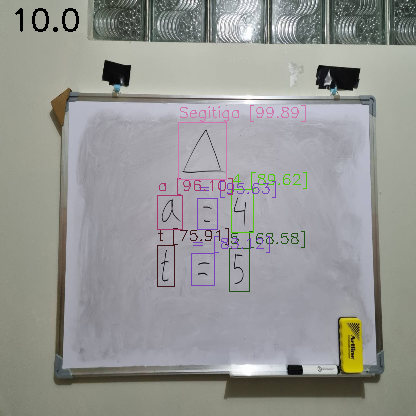
\includegraphics[width=0.55\textwidth]{gambar/seg80hasil.png}
	\captionof{figure}{Deteksi Segitiga dan Hasilnya Pada Pengambilan Gambar 80cm}
	\label{fig:segitigatest80}
\end{center}
Pada Gambar \ref{fig:segitigatest80} didapatkan berhasilnya deteksi daripada gambar bangun datar segitiga beserta parameter huruf dan angka, yang mengakibatkan berhasilnya perhitungan luas yang mana hasil dari perhitungan luas diletakkan pada pojok kiri atas \textit{window} gambar.

\begin{center}
	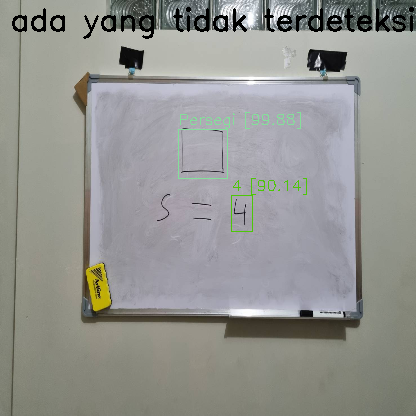
\includegraphics[width=0.55\textwidth]{gambar/pers80hasil.png}
	\captionof{figure}{Deteksi Persegi dan Hasilnya Pada Pengambilan Gambar 80cm}
	\label{fig:persegitest80}
\end{center}
Pada Gambar \ref{fig:persegitest80} didapatkan tidak berhasil sepenuhnya deteksi daripada gambar bangun datar persegi beserta parameter huruf dan angka, yang mengakibatkan tidak berhasilnya perhitungan luas yang mana akan memberikan pesan kesalahan "ada yang tidak terdeteksi".

\begin{center}
	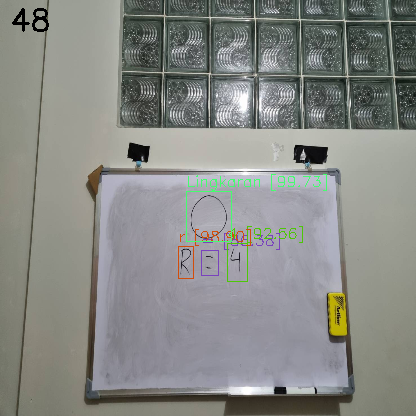
\includegraphics[width=0.55\textwidth]{gambar/ling80hasil.png}
	\captionof{figure}{Deteksi Lingkaran dan Hasilnya Pada Pengambilan Gambar 80cm}
	\label{fig:lingkarantest80}
\end{center}
Pada Gambar \ref{fig:lingkarantest80} didapatkan berhasilnya deteksi daripada gambar bangun datar lingkaran beserta parameter huruf dan angka, yang mengakibatkan berhasilnya perhitungan luas yang mana hasil dari perhitungan luas diletakkan pada pojok kiri atas \textit{window} gambar.

\begin{center}
	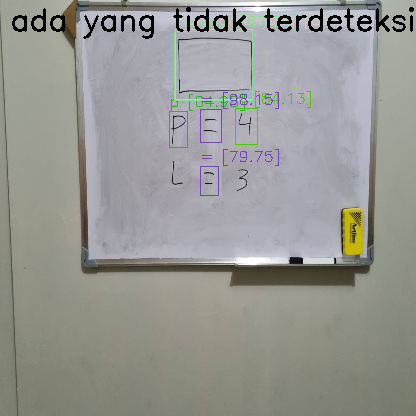
\includegraphics[width=0.55\textwidth]{gambar/pp80hasil.png}
	\captionof{figure}{Deteksi Persegi Panjang dan Hasilnya Pada Pengambilan Gambar 80cm}
	\label{fig:persegipanjangtest80}
\end{center}
Pada Gambar \ref{fig:persegipanjangtest80} didapatkan tidak berhasil sepenuhnya deteksi daripada gambar bangun datar persegi panjang beserta parameter huruf dan angka, yang mengakibatkan tidak berhasilnya perhitungan luas yang mana akan memberikan pesan kesalahan "ada yang tidak terdeteksi".

\begin{center}
	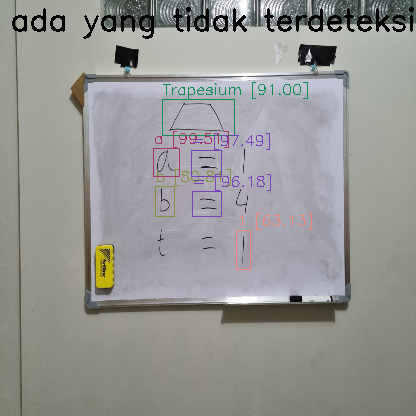
\includegraphics[width=0.55\textwidth]{gambar/trap80hasil.png}
	\captionof{figure}{Deteksi Trapesium dan Hasilnya Pada Pengambilan Gambar 60cm}
	\label{fig:trapesiumtest80}
\end{center}
Pada Gambar \ref{fig:trapesiumtest80} didapatkan tidak berhasil sepenuhnya deteksi daripada gambar bangun datar trapesium beserta parameter huruf dan angka, yang mengakibatkan tidak berhasilnya perhitungan luas yang mana akan memberikan pesan kesalahan "ada yang tidak terdeteksi"

\section{Pengujian menggunakan warna spidol berbeda}
Pada pengujian menggunakanwarna spidol berbeda dilakukan pengujian menggunakan tulisan tangan si peneliti dengan warna spidol yang berbeda, setelah itu dilakukan deteksi objek bangun datar beserta parameternya, dilanjutkan dengan perhitungan luas. Pengujian ini bermaksud untuk melihat seberapa berhasilnya bila model yang sudah di training pada tahap \ref{subsec: Training} di uji coba menggunakan warna spidol yang berbeda. Warna spidol yang digunakan dalam pengujian ini adalah:
\begin{itemize}
	\item Warna spidol biru
	\item Warna spidol merah
	\item Warna spidol hijau
\end{itemize}

\subsection{Pengujian menggunakan warna spidol biru}
\begin{center}
	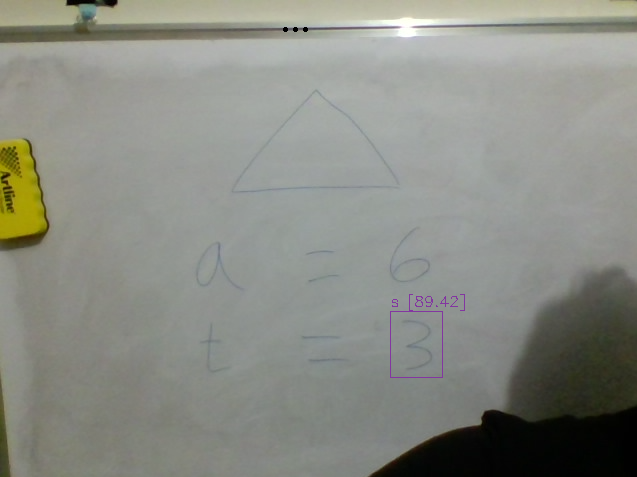
\includegraphics[width=0.55\textwidth]{gambar/segitiga biru.png}
	\captionof{figure}{Deteksi Segitiga dan Hasilnya Pada Pengujian Warna Spidol Biru}
	\label{fig:segitigabiru}
\end{center}
Pada Gambar \ref{fig:segitigabiru} didapatkan tidak berhasilnya deteksi daripada gambar bangun datar segitiga beserta parameter huruf dan angka, yang mengakibatkan tidak berhasilnya perhitungan luas yang mana hasil dari gagalnya perhitungan luas diletakkan pada atas \textit{window} gambar dengan penjelasan "...".

\begin{center}
	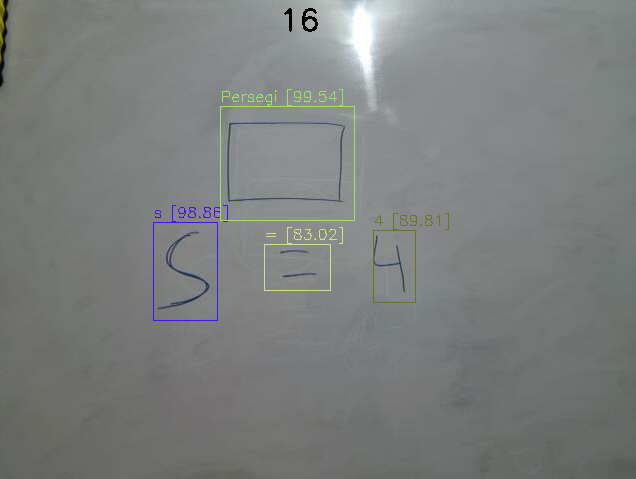
\includegraphics[width=0.55\textwidth]{gambar/persegi biru.png}
	\captionof{figure}{Deteksi Persegi dan Hasilnya Pada Pengujian Warna Spidol Biru}
	\label{fig:persegibiru}
\end{center}
Pada Gambar \ref{fig:persegibiru} didapatkan berhasilnya deteksi daripada gambar bangun datar persegi beserta parameter huruf dan angka, yang mengakibatkan berhasilnya perhitungan luas yang mana hasil dari perhitungan luas diletakkan pada atas \textit{window} gambar.

\begin{center}
	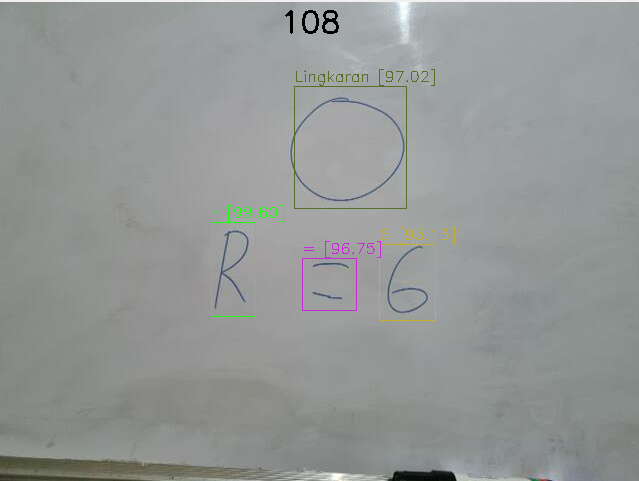
\includegraphics[width=0.55\textwidth]{gambar/lingkaran biru.png}
	\captionof{figure}{Deteksi Lingkaran dan Hasilnya Pada Pengujian Warna Spidol Biru}
	\label{fig:lingkaranbiru}
\end{center}
Pada Gambar \ref{fig:lingkaranbiru} didapatkan berhasilnya deteksi daripada gambar bangun datar lingkaran beserta parameter huruf dan angka, yang mengakibatkan berhasilnya perhitungan luas yang mana hasil dari perhitungan luas diletakkan pada atas \textit{window} gambar.

\begin{center}
	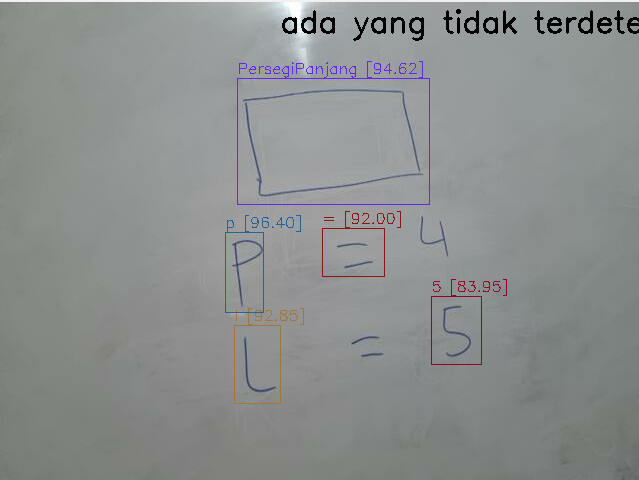
\includegraphics[width=0.55\textwidth]{gambar/persegipanjang biru.png}
	\captionof{figure}{Deteksi Persegi Panjang dan Hasilnya Pada Pengujian Warna Spidol Biru}
	\label{fig:ppbiru}
\end{center}
Pada Gambar \ref{fig:ppbiru} didapatkan tidak berhasilnya deteksi daripada gambar bangun datar persegi panjang beserta parameter huruf dan angka, yang mengakibatkan tidak berhasilnya perhitungan luas yang mana hasil dari gagalnya perhitungan luas diletakkan pada atas \textit{window} gambar dengan penjelasan "ada yang tidak terdeteksi".

\begin{center}
	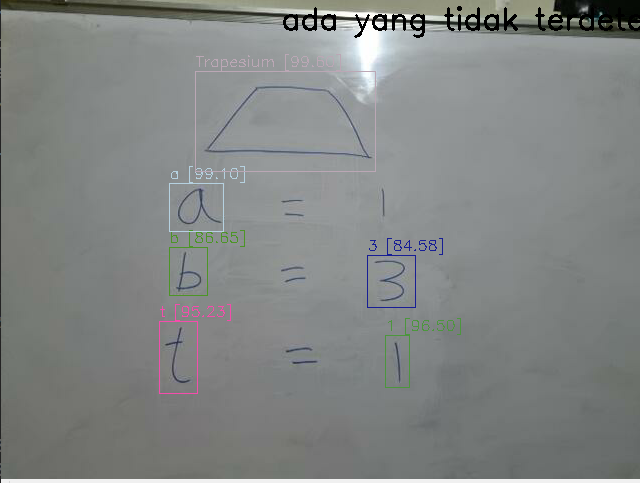
\includegraphics[width=0.55\textwidth]{gambar/trapesium biru.png}
	\captionof{figure}{Deteksi Trapesium dan Hasilnya Pada Pengujian Warna Spidol Biru}
	\label{fig:trapbiru}
\end{center}
Pada Gambar \ref{fig:trapbiru} didapatkan tidak berhasilnya deteksi daripada gambar bangun datar trapesium beserta parameter huruf dan angka, yang mengakibatkan tidak berhasilnya perhitungan luas yang mana hasil dari gagalnya perhitungan luas diletakkan pada atas \textit{window} gambar dengan penjelasan "ada yang tidak terdeteksi".

\subsection{Pengujian menggunakan warna spidol merah}
\begin{center}
	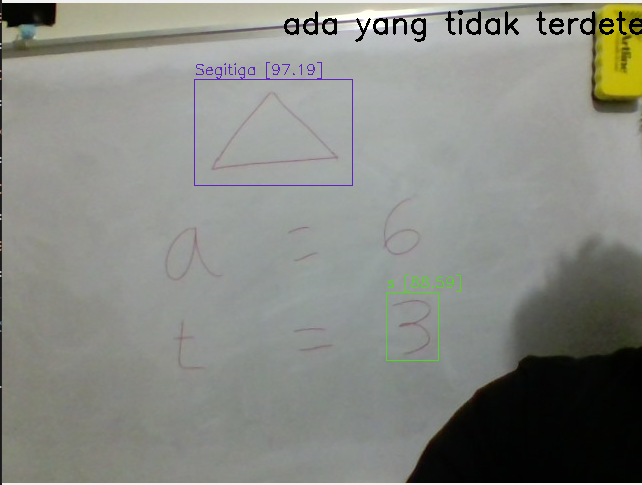
\includegraphics[width=0.55\textwidth]{gambar/segitiga merah.png}
	\captionof{figure}{Deteksi Segitiga dan Hasilnya Pada Pengujian Warna Spidol Merah}
	\label{fig:segitigamerah}
\end{center}
Pada Gambar \ref{fig:segitigamerah} didapatkan tidak berhasilnya deteksi daripada gambar bangun datar segitiga beserta parameter huruf dan angka, yang mengakibatkan tidak berhasilnya perhitungan luas yang mana hasil dari gagalnya perhitungan luas diletakkan pada atas \textit{window} gambar dengan penjelasan "ada yang tidak teredeteksi".

\begin{center}
	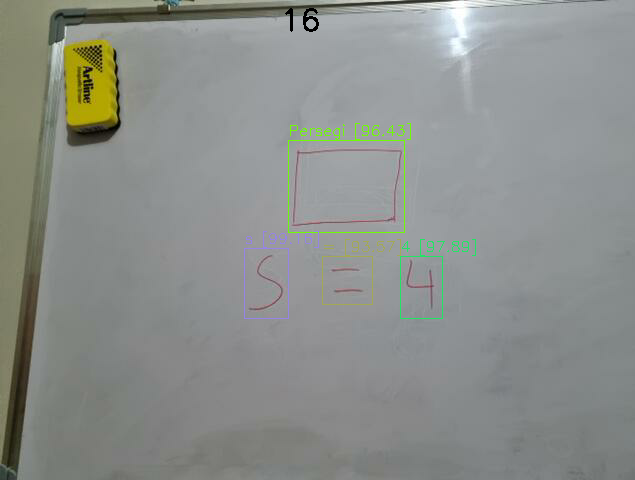
\includegraphics[width=0.55\textwidth]{gambar/persegi merah.png}
	\captionof{figure}{Deteksi Persegi dan Hasilnya Pada Pengujian Warna Spidol Merah}
	\label{fig:persegimerah}
\end{center}
Pada Gambar \ref{fig:persegimerah} didapatkan berhasilnya deteksi daripada gambar bangun datar persegi beserta parameter huruf dan angka, yang mengakibatkan berhasilnya perhitungan luas yang mana hasil dari perhitungan luas diletakkan pada atas \textit{window} gambar.

\begin{center}
	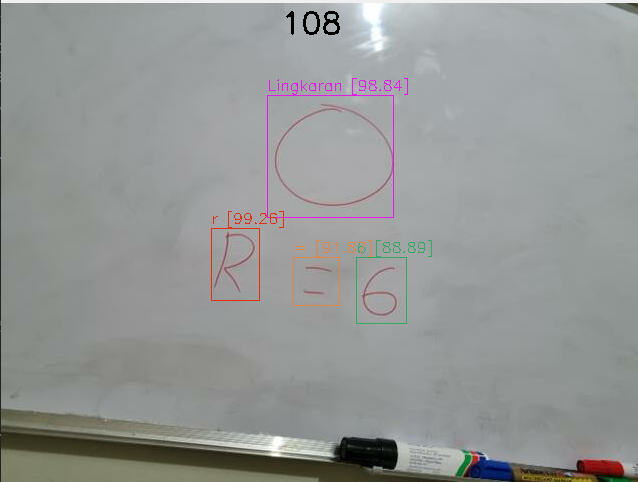
\includegraphics[width=0.55\textwidth]{gambar/lingkaran merah.png}
	\captionof{figure}{Deteksi Lingkaran dan Hasilnya Pada Pengujian Warna Spidol Merah}
	\label{fig:lingkaranmerah}
\end{center}
Pada Gambar \ref{fig:lingkaranmerah} didapatkan berhasilnya deteksi daripada gambar bangun datar lingkaran beserta parameter huruf dan angka, yang mengakibatkan berhasilnya perhitungan luas yang mana hasil dari perhitungan luas diletakkan pada atas \textit{window} gambar.

\begin{center}
	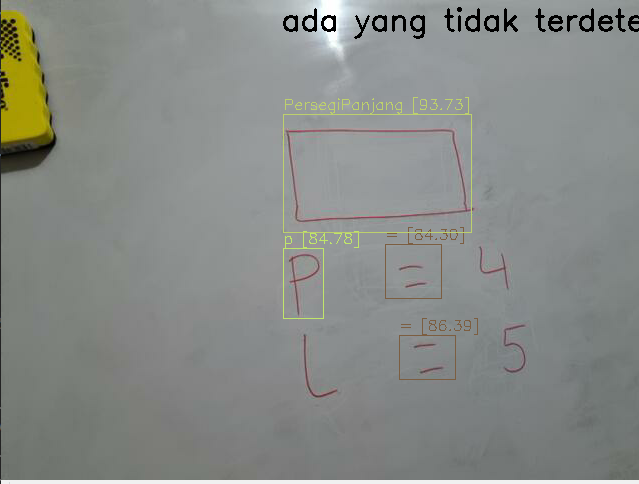
\includegraphics[width=0.55\textwidth]{gambar/persegipanjang merah.png}
	\captionof{figure}{Deteksi Persegi Panjang dan Hasilnya Pada Pengujian Warna Spidol Merah}
	\label{fig:ppmerah}
\end{center}
Pada Gambar \ref{fig:ppmerah} didapatkan tidak berhasilnya deteksi daripada gambar bangun datar persegi panjang beserta parameter huruf dan angka, yang mengakibatkan tidak berhasilnya perhitungan luas yang mana hasil dari gagalnya perhitungan luas diletakkan pada atas \textit{window} gambar dengan penjelasan "ada yang tidak terdeteksi".

\begin{center}
	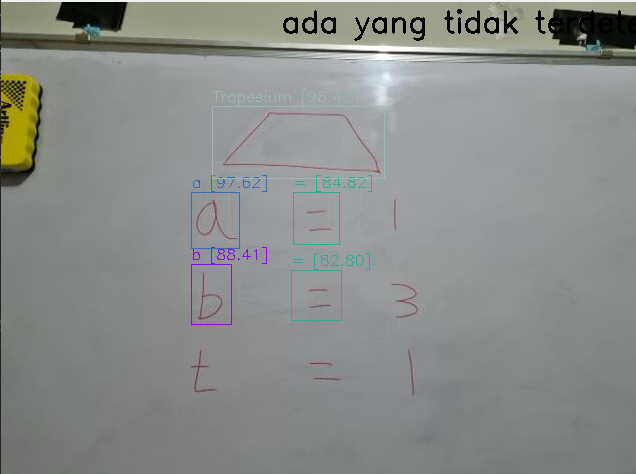
\includegraphics[width=0.55\textwidth]{gambar/trapesium merah.png}
	\captionof{figure}{Deteksi Trapesium dan Hasilnya Pada Pengujian Warna Spidol Merah}
	\label{fig:trapmerah}
\end{center}
Pada Gambar \ref{fig:trapmerah} didapatkan tidak berhasilnya deteksi daripada gambar bangun datar trapesium beserta parameter huruf dan angka, yang mengakibatkan tidak berhasilnya perhitungan luas yang mana hasil dari gagalnya perhitungan luas diletakkan pada atas \textit{window} gambar dengan penjelasan "ada yang tidak terdeteksi".

\subsection{Pengujian menggunakan warna spidol hijau}
\begin{center}
	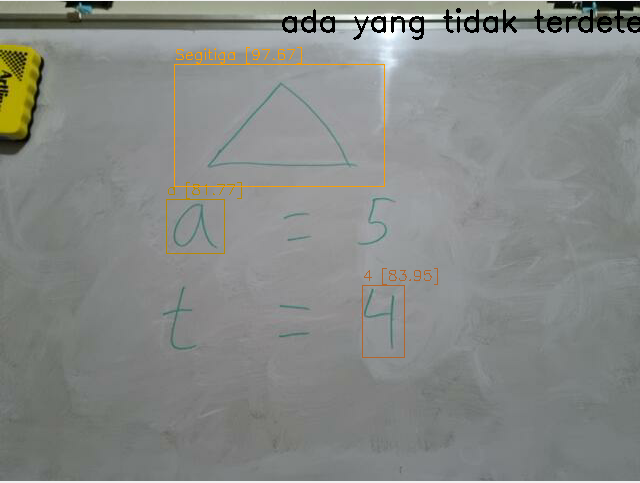
\includegraphics[width=0.55\textwidth]{gambar/segitiga hijau.png}
	\captionof{figure}{Deteksi Segitiga dan Hasilnya Pada Pengujian Warna Spidol Hijau}
	\label{fig:segitigahijau}
\end{center}
Pada Gambar \ref{fig:segitigahijau} didapatkan tidak berhasilnya deteksi daripada gambar bangun datar segitiga beserta parameter huruf dan angka, yang mengakibatkan tidak berhasilnya perhitungan luas yang mana hasil dari gagalnya perhitungan luas diletakkan pada atas \textit{window} gambar dengan penjelasan "ada yang tidak teredeteksi".

\begin{center}
	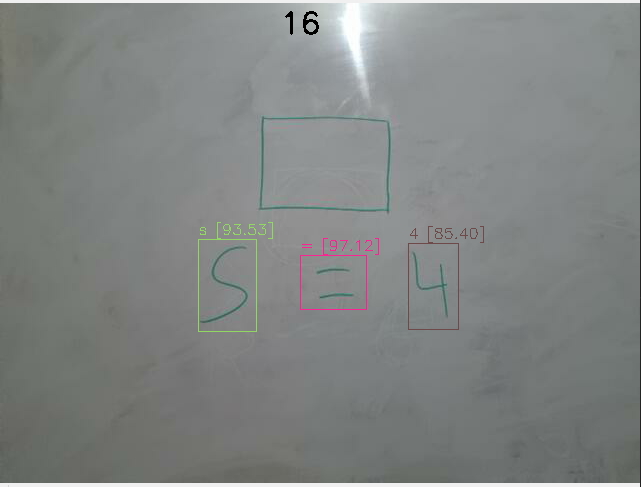
\includegraphics[width=0.55\textwidth]{gambar/persegi hijau.png}
	\captionof{figure}{Deteksi Persegi dan Hasilnya Pada Pengujian Warna Spidol Hijau}
	\label{fig:persegihijau}
\end{center}
Pada Gambar \ref{fig:persegihijau} didapatkan berhasilnya deteksi daripada gambar bangun datar persegi beserta parameter huruf dan angka, yang mengakibatkan berhasilnya perhitungan luas yang mana hasil dari perhitungan luas diletakkan pada atas \textit{window} gambar.

\begin{center}
	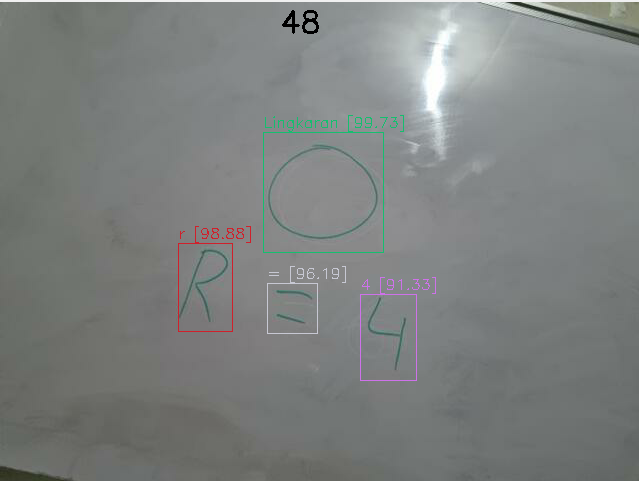
\includegraphics[width=0.55\textwidth]{gambar/lingkaran hijau.png}
	\captionof{figure}{Deteksi Lingkaran dan Hasilnya Pada Pengujian Warna Spidol Hijau}
	\label{fig:lingkaranhijau}
\end{center}
Pada Gambar \ref{fig:lingkaranhijau} didapatkan berhasilnya deteksi daripada gambar bangun datar lingkaran beserta parameter huruf dan angka, yang mengakibatkan berhasilnya perhitungan luas yang mana hasil dari perhitungan luas diletakkan pada atas \textit{window} gambar.

\begin{center}
	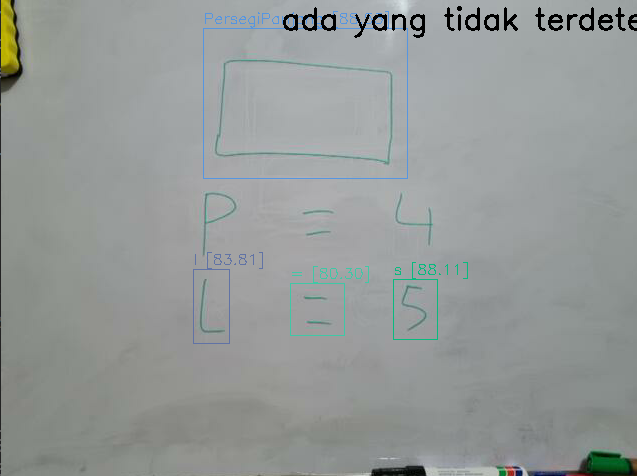
\includegraphics[width=0.55\textwidth]{gambar/persegipanjang hijau.png}
	\captionof{figure}{Deteksi Persegi Panjang dan Hasilnya Pada Pengujian Warna Spidol Hijau}
	\label{fig:pphijau}
\end{center}
Pada Gambar \ref{fig:pphijau} didapatkan tidak berhasilnya deteksi daripada gambar bangun datar persegi panjang beserta parameter huruf dan angka, yang mengakibatkan tidak berhasilnya perhitungan luas yang mana hasil dari gagalnya perhitungan luas diletakkan pada atas \textit{window} gambar dengan penjelasan "ada yang tidak terdeteksi".

\begin{center}
	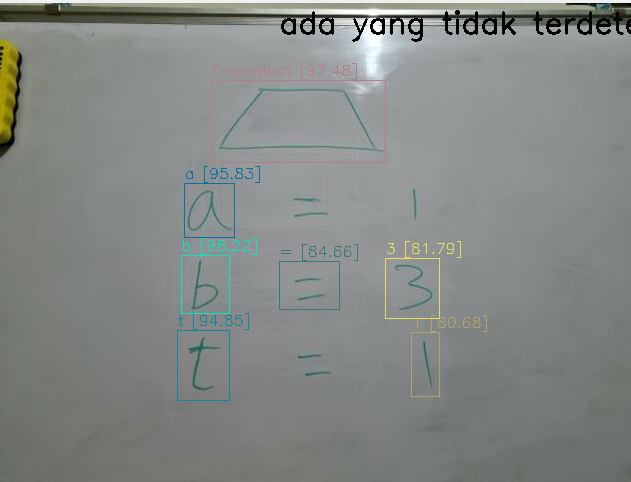
\includegraphics[width=0.55\textwidth]{gambar/trapesium hijau.png}
	\captionof{figure}{Deteksi Trapesium dan Hasilnya Pada Pengujian Warna Spidol Hijau}
	\label{fig:traphijau}
\end{center}
Pada Gambar \ref{fig:traphijau} didapatkan tidak berhasilnya deteksi daripada gambar bangun datar trapesium beserta parameter huruf dan angka, yang mengakibatkan tidak berhasilnya perhitungan luas yang mana hasil dari gagalnya perhitungan luas diletakkan pada atas \textit{window} gambar dengan penjelasan "ada yang tidak terdeteksi".

\section{Pengujian menggunakan gambar bangun datar yang diarsir}
Pada pengujian menggunakan gambar bangun datar yang diarsir dilakukan pengujian menggunakan tulisan tangan si peneliti dengan gambar bangun datar yang diarsir, setelah itu dilakukan deteksi objek bangun datar beserta parameternya, dilanjutkan dengan perhitungan luas. Pengujian ini bermaksud untuk melihat seberapa berhasilnya bila model yang sudah di training pada tahap \ref{subsec: Training} di uji coba menggunakan gambar bangun datar yang diarsir.

\begin{center}
	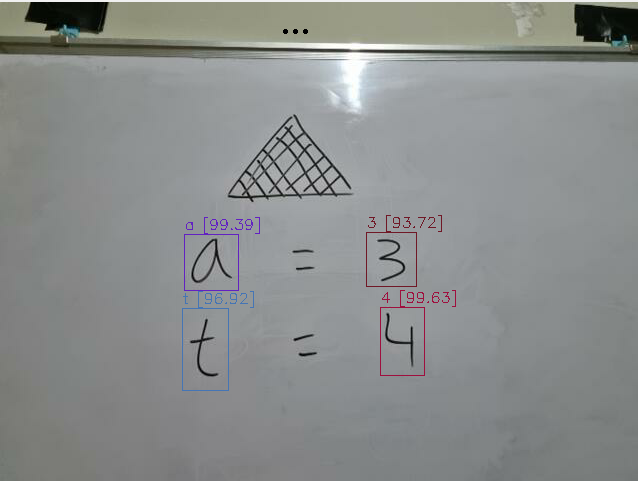
\includegraphics[width=0.55\textwidth]{gambar/segitiga arsir.png}
	\captionof{figure}{Deteksi Segitiga dan Hasilnya Pada Pengujian Gambar Arsir}
	\label{fig:segitigaarsir}
\end{center}
Pada Gambar \ref{fig:segitigaarsir} didapatkan tidak berhasilnya deteksi daripada gambar bangun datar segitiga beserta parameter huruf dan angka, yang mengakibatkan tidak berhasilnya perhitungan luas yang mana hasil dari gagalnya perhitungan luas diletakkan pada atas \textit{window} gambar dengan penjelasan "...".

\begin{center}
	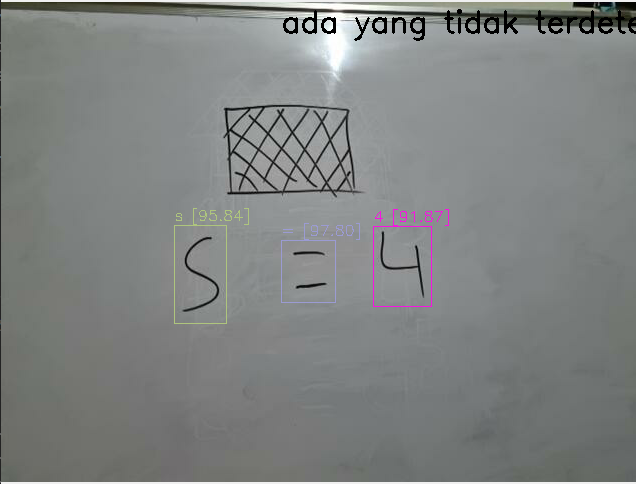
\includegraphics[width=0.55\textwidth]{gambar/persegi arsir.png}
	\captionof{figure}{Deteksi Persegi dan Hasilnya Pada Pengujian Gambar Arsir}
	\label{fig:persegiarsir}
\end{center}
Pada Gambar \ref{fig:persegiarsir} didapatkan tidak berhasilnya deteksi daripada gambar bangun datar persegi beserta parameter huruf dan angka, yang mengakibatkan tidak berhasilnya perhitungan luas yang mana hasil dari gagalnya perhitungan luas diletakkan pada atas \textit{window} gambar dengan penjelasan "ada yang tidak terdeteksi".

\begin{center}
	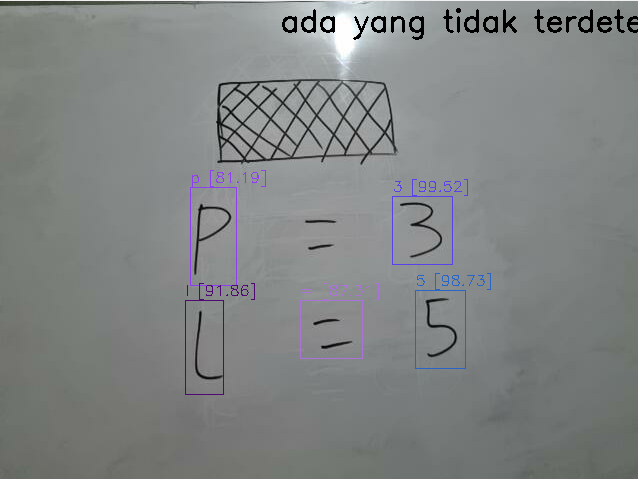
\includegraphics[width=0.55\textwidth]{gambar/persegipanjang arsir.png}
	\captionof{figure}{Deteksi Persegi Panjang dan Hasilnya Pada Pengujian Gambar Arsir}
	\label{fig:pparsir}
\end{center}
Pada Gambar \ref{fig:pparsir} didapatkan tidak berhasilnya deteksi daripada gambar bangun datar persegi panjang beserta parameter huruf dan angka, yang mengakibatkan tidak berhasilnya perhitungan luas yang mana hasil dari gagalnya perhitungan luas diletakkan pada atas \textit{window} gambar dengan penjelasan "ada yang tidak terdeteksi".

\begin{center}
	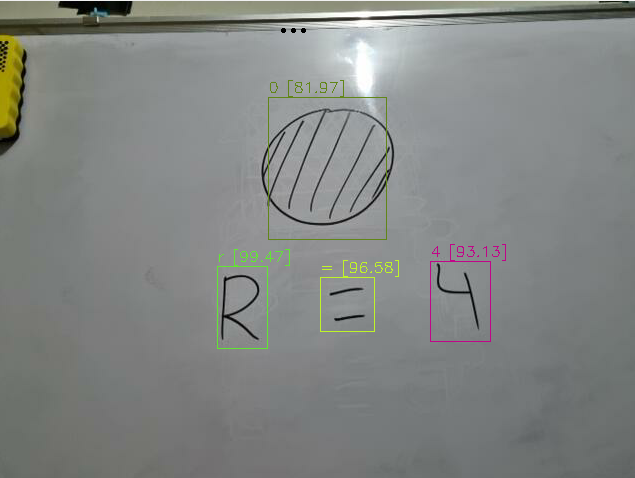
\includegraphics[width=0.55\textwidth]{gambar/lingkaran arsir.png}
	\captionof{figure}{Deteksi lingkaran dan Hasilnya Pada Pengujian Gambar Arsir}
	\label{fig:lingkaranarsir}
\end{center}
Pada Gambar \ref{fig:lingkaranarsir} didapatkan tidak berhasilnya deteksi daripada gambar bangun datar lingkaran beserta parameter huruf dan angka, yang mengakibatkan tidak berhasilnya perhitungan luas yang mana hasil dari gagalnya perhitungan luas diletakkan pada atas \textit{window} gambar dengan penjelasan "...".

\begin{center}
	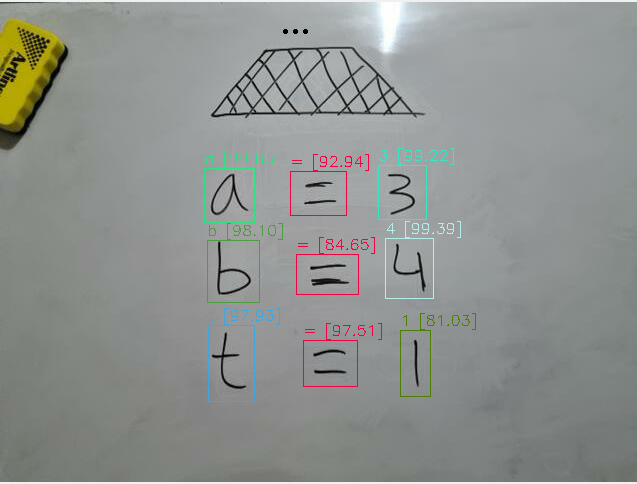
\includegraphics[width=0.55\textwidth]{gambar/trapesium arsir.png}
	\captionof{figure}{Deteksi Trapesium dan Hasilnya Pada Pengujian Gambar Arsir}
	\label{fig:traparsir}
\end{center}
Pada Gambar \ref{fig:traparsir} didapatkan tidak berhasilnya deteksi daripada gambar bangun datar trapesium beserta parameter huruf dan angka, yang mengakibatkan tidak berhasilnya perhitungan luas yang mana hasil dari gagalnya perhitungan luas diletakkan pada atas \textit{window} gambar dengan penjelasan "...".

\section{Hasil Training}
Dalam penelitian ini, platform yang digunakan dalam penulisan ini adalah platform software Visual Studio Code, CUDA 11.5, cuDNN 8.3.2, OpenCV 4.5.4 dan GPU Nvidia GeForce 1060. Operasi sistem yang digunakan adalah Windows 10 serta \textit{framework} Darknet Network. Versi YOLO yang digunakan adalah YOLOv4-tiny.

Data yang digunakan sebanyak 807 gambar yang terdiri dari 726 data \textit{training} dan 81 data \textit{testing}. Data training dilakukan dengan epoch 10000 sampai epoch 40000. Pengujian dilakukan dengan pengambilan data \textit{True Positives} (TP), \textit{False Positive} (FP), dan \textit{False Negative} (FN). TP adalah objek gambar bangun datar dan parameternya dari gambar yang berhasil dideteksi oleh algoritma YOLO. FP adalah objek yang salah terdeteksi sebagai objek gambar bangun datar dan parameternya. FN adalah ketika algoritma tidak dapat mengenali objek gambar bangun datar dan parameternya dalam gambar. Dari nilai TP, FP dan FN dapat diperoleh nilai \textit{f-1 score}, \textit{Precision}, dan \textit{Recall} dengan rumus sebagai berikut: \\
Hasil dari 10000 epoch sampai 40000 epoch dapat dilihat pada Tabel berikut.

\begin{table}[H]
	\centering
	\begin{tabular}{c c c c} 
		\toprule
		Epoch & TP & FP & FN \\ [0.5ex] 
		\midrule
		10000 & 3125 & 26 & 9 \\ 
		\midrule
		20000 & 3119 & 24 & 15 \\
		\midrule
		30000 & 3128 & 14 & 6 \\
		\midrule
		40000 & 3124 & 14 & 10 \\ [1ex] 
		\bottomrule
	\end{tabular}
	\caption{TP,FP, FN pada tiap epoch}
\end{table}

Berdasarkan tabel nilai TP tertinggi pada jumlah epoch 30000 adalah 3128. Nilai FP dan FN terendah juga pada total epoch 30000 yaitu masing-masing 14 dan 6. Dengan demikian, deteksi objek tulisan tangan pada papan tulis terbaik saat epoch mencapai 30000. Nilai \textit{f1-score}, \textit{Precision}, dan \textit{Recall} didapatkan dengan rumus berikut.
\textit{Precision}: $$\frac{TP}{TP+FP}$$\\
\textit{Recall}: $$\frac{TP}{TP+FN}$$\\
\textit{F1-Score}: $$2*\frac{\textit{Precision}*\textit{Recall}}{\textit{Precision}+\textit{Recall}}$$\\
dengan menerapkan rumus yang ada, maka didapatkan nilai \textit{f1-score}, \textit{Precision}, dan \textit{Recall} yang ditunjukkan pada tabel berikut.
\begin{table}[H]
	\centering
	\begin{tabular}{c c c c}
		\toprule
		Epoch & Presisi & Recall  & F1-score \\
		\midrule
		10000 & 99,17\% & 99,71\% & 99,44\%  \\
		\midrule
		20000 & 99,23\% & 99,52\% & 99,37\%  \\
		\midrule
		30000 & 99,55\% & 99,80\% & 99,68\%  \\
		\midrule
		40000 & 99,55\% & 99,68\% & 99,61\% \\
		\bottomrule
	\end{tabular}
	\caption{Presisi, Recall, dan F1-score pada tiap epoch}
\end{table}